\documentclass[11pt]{article}
\usepackage[utf8]{inputenc}
\usepackage[margin=1in]{geometry}
\usepackage{amsmath,amssymb}
\usepackage{multicol}
\usepackage{enumerate}
\usepackage{graphicx}
\usepackage{spalign}
\usepackage{hyperref}
\setlength{\parindent}{0pt}
\usepackage{listings} 
\usepackage{mdframed}
\usepackage{systeme}
\usepackage{amsmath}
\usepackage[colorinlistoftodos]{todonotes}
\usepackage{amssymb}
\usepackage{marginnote}
\usepackage{float}
\usepackage{subfig}
\usepackage{enumerate}
\usepackage{amsfonts}
\usepackage{amssymb}
\usepackage{mathrsfs}
\usepackage{dsfont}
\usepackage{algorithm}
\usepackage{algpseudocode}
\usepackage{pifont}
%\usepackage[table,xcdraw]{xcolor}

\title{Modeling Rumour Spread}
\author{Nicholas Mankowski}
\date{December 13th, 2023}


%%	 MATLAB
\usepackage[framed,numbered,autolinebreaks,useliterate]{mcode}


\renewcommand{\theenumi}{\Alph{enumi}}
\newcommand{\phanmin}{\phantom{-}}
\renewcommand{\vec}[1]{\mathbf{#1}}

\lstset{
  columns=fullflexible,
  keepspaces=true,
  literate={delta}{{\text{delta}}}1
}

\begin{document}

\maketitle

%\rule[2ex]{\textwidth}{2pt}

\large
\section{Introduction}
A rumour has started to spread at Ohio Wesleyan.  
The rumour is that Ohio Wesleyan's premier fraternity, Oozma Kappa, will not have their annual pumpkin carving contest due to a shortage of pumpkins in the Delaware area.  
This is of course not true, as farmers indicate a spectacularly average year for pumpkin crop yields.  
This rumour is being spread by Dr. McCurdy in the math department, as he wants revenge against Dr. Guo's show-stopping pumpkin from last year.  
Dr. McCurdy cannot begin to think what will happen if he loses the pumpkin carving contest two years in a row, so he has no other option than to try and stop the event.
Dr. McCurdy begins spreading this rumour in his math modeling class, but some of the students in this class do not believe the rumour and do not spread it, while others in the class are telling everybody around the school.
These reactions are rather telling, and offer us a glimpse into how the rumour will spread across the university.
In this writeup, we will explore how Dr. McCurdy's rumour will spread around the campus population by using SIR-like modeling techniques.

\section{Description of Mathematics}
We will use a variation of the SIR modeling technique to analyze the spread of the rumour throughout Ohio Wesleyan.  
We can create three different categories to describe the possible status of a student/faculty member at Ohio Wesleyan.
These categories are as follows:
\begin{itemize}
    \item $H$: Somebody who has heard the rumour, and is actively spreading it.
    \item $I$: Somebody who has not heard the rumour.
    \item $R$: Somebody who has heard rumour, but is refusing to spread it.
\end{itemize}

We can represent the pathways between the different statuses of people as the following:
\begin{itemize}
    \item $H \rightarrow I$: People who were spreading the rumour, but have forgotten the rumour.  This is purely dependent on the number of people who are spreading the rumour, so we can describe this rate as $\delta H$.
    \item $H \rightarrow R$: People who were spreading the rumour, but have since refused.  This is dependent on the number of people who are spreading the rumour, so we can describe this rate as $\beta H$.
    \item $I \rightarrow H$: People who have heard the rumour and begin to spread it.  This is dependent on the interaction between people who have heard the rumour and those who haven't, so we can describe this rate as $\alpha I H$.
    \item $R \rightarrow H$: People who have previously refused to spread the rumour, but begin to spread it.  This is dependent solely on the number of people who refuse to spread the rumour, so we can describe this rate as $\varepsilon R$.
    \item $R \rightarrow I$: People who were refusing to spread the rumour, but have since forgotten it.  This is purely dependent on the number of people who are currently refusing to spread the rumour, so we can describe this rate as $\gamma R$.
\end{itemize}
With this information, we can represent our model as the following graph:
\begin{figure}[H]
    \centering
    \caption{HIR Model Diagram}
    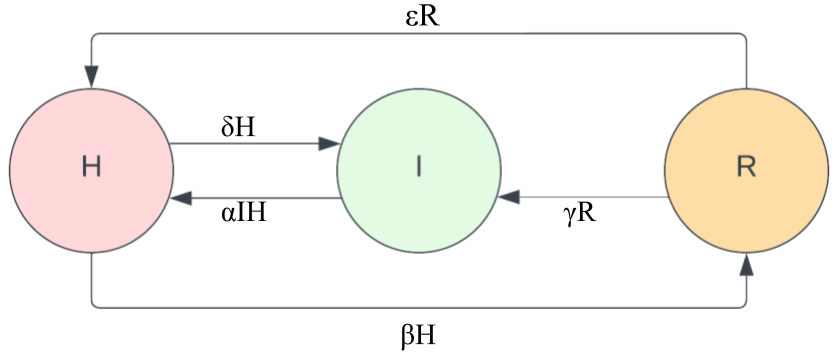
\includegraphics[width=0.8\columnwidth]{models/HIR_Model.png}
    \label{HIR-diagram}
\end{figure}
Using this model, we can set up three differential equations to represent the rate of change for each node.  
Doing this, we have the following system of differential equations:
\begin{align*}
    \frac{d H}{d t} & = \varepsilon R + \alpha I H - \delta H - \beta H & = \varepsilon R + \alpha I H - (\delta + \beta) H \\ % TODO: verify these
    \frac{d I}{d t} & & = \delta H + \gamma R - \alpha I H \\
    \frac{d R}{d t} & = \beta H - \varepsilon R - \gamma R & = \beta H - (\varepsilon + \gamma) R.
\end{align*}
While this system of differential equations may be difficult or even impossible to solve analytically, we are able to discretize the equations to produce an approximate solution to the system.
This technique has the added benefit that all systems will have a similar approach in solving and will not depend on the equations themselves, as is often the case with solving differential equations analytically.
In order to produce this approximation, we must convert our continuous differential equations to discrete difference equations.  
Doing this, we have
\begin{align*}
    \frac{\Delta H}{\Delta t} & = \frac{H(t + \Delta t) - H(t)}{\Delta t} = \varepsilon R(t) + \alpha I(t) H(t) - (\delta + \beta) H(t) \\% TODO: fix these
    \frac{\Delta I}{\Delta t} & = \frac{I(t + \Delta t) - I(t)}{\Delta t} = \delta H(t) + \gamma R(t) - \alpha I(t) H(t) \\
    \frac{\Delta R}{\Delta t} & = \frac{R(t + \Delta t) - R(t)}{\Delta t} = \beta H(t) - (\varepsilon + \gamma)R(t),    
\end{align*}


where $t$ is our current time, $\Delta t$ is our discrete time step, $\Delta H$ is our discrete step in $H$, $\Delta I$ is our discrete step in $I$, and $\Delta R$ is our discrete step in $R$. \\

Now that we have a discretized system, we can solve each difference equation to give us the next time step using the data from the previous time step.  Doing this, we obtain
\label{change-eqs}
\begin{align*}
    H(t + \Delta t) & = \Delta t(\varepsilon R(t) + \alpha I(t) H(t) - (\delta + \beta - 1) H(t)) \\ % TODO: fix these
    I(t + \Delta t) & = \Delta t(\delta H(t) + \gamma R(t) - \alpha I(t) H(t)) + I(t) \\
    R(t + \Delta t) & = \Delta t(\beta H(t) - (\varepsilon + \gamma - 1) R(t), 
\end{align*}
which gives us an estimation of our differential equation solution.  Using this, we can find our approximate curves iteratively given an initial condition.

\section{Applications in Code} \label{applications-in-code}
Given our explicit discretized equations derived in \ref{change-eqs}, we can iterate through values using a \texttt{for} loop in MATLAB in order to produce an approximate solution to our system of differential equations.
In order to accomplish this, we must first declare our parameters $\alpha, \beta, \gamma, \; \& \; \varepsilon$.
We can accomplish this as follows:
\begin{lstlisting}
% Set up parameters
alpha = 0.001;
beta = 0.04;
gamma = 0.01;
delta = 0.01;
epsilon = 0.005;
\end{lstlisting}
Now that we have our parameters set up, we can create our corresponding variables to handle time.  
To do this, we will need an initial time, a maximum time, and a time step. 
We will take our initial time to be $0$, our maximum time to be $100$, and our time step to be $1$.  
We do this as follows:
\begin{lstlisting}
% Set up time variables
deltaT = 1; % Time step
startTime = 0; % Initial time
maxTime = 100; % Maximum time(non inclusive)
\end{lstlisting}
\textbf{Note:} We do not want our maximum time to be inclusive, since we are counting from zero.
If we set up our maximum time to be inclusive, we will have a mismatch in array lengths when plotting our solution. \\ \\
In order to set up our vectors to ultimately hold our approximations, we must create a vector for each value that holds $\frac{t_{\text{max}} - t_{\text{min}}}{\Delta t}$ values where $t_{\text{max}}$ is the maximum time value and $t_{\text{min}}$ is the minimum time value.
So, we declare our vectors as the following:
\begin{lstlisting}
% Set up arrays that will hold our values of H, I, & R.
H = ones(1, (maxTime - startTime) / deltaT);
I = ones(1, (maxTime - startTime) / deltaT);
R = ones(1, (maxTime - startTime) / deltaT);
\end{lstlisting}

Now, we must set up our initial conditions.  
Unfortunately, due to low enrollment numbers, Ohio Wesleyan has a total of 200 students and faculty.  Thus, we must have 199 people unaware of the rumour and 1 person (Dr. McCurdy) spreading the rumour initially.
This also means that we initially have nobody refusing to spread the rumour.  
Thus, we can set up our vectors containing our data and their initial conditions as follows:
\begin{lstlisting}
H(1) = 1; % The original person spreading the rumour
I(1) = 199; % Initial population of people not spreading rumour
R(1) = 0;
\end{lstlisting}

Now that we have our initial conditions set up, we are able to iterate through our difference equations to produce an approximation of our solution.
We can do this in MATLAB by doing the following:
\begin{lstlisting}
% Iterate through each time step.  
% We must exclude the last value, since we are setting the value at t + 1, 
% so iterating until length(H) would cause us to go out of bounds.
for t = 1:length(H) - 1
    % Calculate the next value of H, I, & R based on the previous values using our difference equations.
    H(t + 1) = deltaT * (epsilon * R(t) + alpha * I(t) * H(t) - (delta + beta) * H(t)) + H(t);
    I(t + 1) = deltaT * (delta * H(t) + gamma * R(t) - alpha * I(t) * H(t)) + I(t);
    R(t + 1) = deltaT * (beta * H(t) - (epsilon + gamma) * R(t)) + R(t);
end
\end{lstlisting}
Now that we have assembled our model, we can plot $H, I, \; \& \; R$ by creating a representation of continuous time and plotting against this.
Doing this, we have the following:
\begin{lstlisting}
% "Continuous" time, subtract deltaT since we do not want it to be inclusive.
% If we make this inclusive, it will cause errors in the length of our H, I, & R vectors,
% since we are counting from zero.
timeCts = startTime:deltaT:maxTime - deltaT; 
    
% Plot the model
hold on;
% Plot H, I, & R
plot(timeCts, H, 'DisplayName', 'H, students actively spreading the rumour');
plot(timeCts, I, 'DisplayName', 'I, students ignorant to the rumour');
plot(timeCts, R, 'DisplayName', 'R, students refusing to spread the rumour');
% Label the graph and add a legend
xlabel('Time (t)')
ylabel('Population')
title('Rumour Spread Across OWU Campus and Faculty')
legend;
hold off;
\end{lstlisting}

\section{Discussion}
By following the methodology described in \ref{applications-in-code}, we produce the following graph:
\begin{figure}[H]
    \centering
    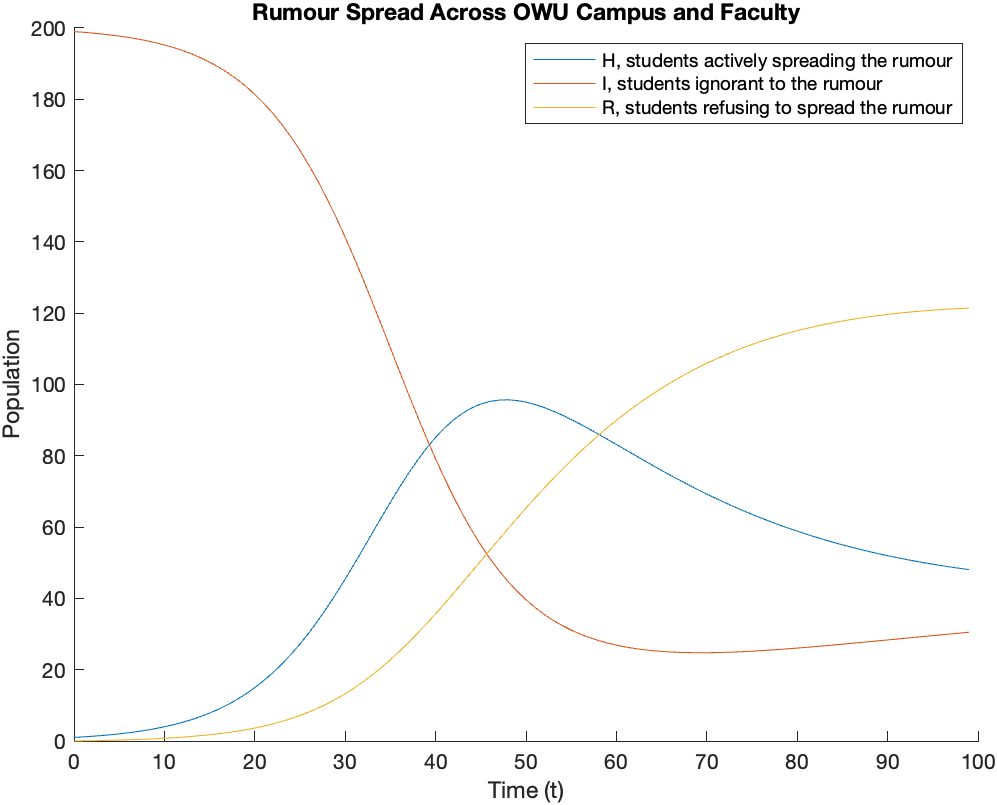
\includegraphics[width=0.8\columnwidth,keepaspectratio]{models/model.png}
    \caption{Rumour Spread Model}
    \label{model-graph}
\end{figure}

\subsection{Parameter Analysis}
We can look at the effect that the parameters will have on our model by digging a bit deeper into the underlying math we had established and using a bit of intuition.
Via the results shown in \ref{model-graph}, we can see that the parameters,
\begin{equation*}
\label{model-parameters}
\alpha = 0.001 \, , \quad \beta = 0.04 \, , \quad \gamma = 0.01 \, , \quad \delta = 0.01 \, , \quad \varepsilon = 0.005 \, ,
\end{equation*}
produce realistic curves that can be used to approximate the rumour spread. 
Further examining these parameters, we should note that their order is closely related to the time scale that we are looking at.
For example, $\alpha = 0.001$ moves significantly more people if we are looking at a larger span of time than a smaller one.
This relation to the arbitrary time scale means that we should moreso focus on the relationships between these parameters, rather than their exact values.
Looking at our paremeters, $\gamma = 0.01$ and $\beta = 0.04$ implies that ignorant people hearing about the rumour are much less likely to spread the rumour than they are to refuse to spread it.
Thus, we are assuming our population to be fairly resistant to spreading the rumour.
Similarly, $\varepsilon = 0.005$ and $\gamma = 0.01$ means that the population of people refusing to spread the rumour are much more likely to forget about the rumour than they are to begin spreading it.
Overall, the ratios between these parameter values seem to match intuition regarding what masses of people will do when facing a rumour.
Thus, they are reasonable for this model.
\\

Looking at our graphic first shown in \ref{HIR-diagram}, we can draw some conclusions about how changing our model parameters will affect our model.
We can create the following conclusions based on this:
\begin{itemize}
    \item By increasing/decreasing the value of $\alpha$, we are altering the percentage of interactions between a rumour spreading student and an ignorant student that will cause that ignorant student to learn of the rumour.  If we are to increase this value, it will cause more people to spread the rumour, but also could cause more people to refuse spreading the rumour via the pathway from $H \rightarrow R$.
    \item By increasing/decreasing the value of $\beta$, we are changing the percentage of rumour spreading students that eventually refuse to spread the rumour at each time step.  A high value for this will cause less people to be spreading the rumour and more people to be refusing to spread the rumour.  This is because a high $\beta$ value will cause more people to flow across the pathway $H \rightarrow R$ and thus more people will refuse to spread the rumour who were previously actively spreading the rumour.
    \item By increasing/decreasing the value of $\gamma$, we are changing the rate at which people forget the rumour among those not actively spreading it.  By having a higher $\gamma$ value, there will be fewer people who are refusing to spread the rumour and more people ignorant to the rumour.  This may seem to not have an effect, but a larger amount of ignorant people could possibly mean more people eventually spreading the rumour, so having this value be very large may have the effect of increasing the number of people spreading the rumour.
    \item By increasing/decreasing the value of $\delta$, we are causing more people who are actively spreading the rumour to forget it.  This rate is likely very small, as it is unlikely that somebody spreading the rumour would forget it, but a higher $\delta$ value will likely lead to more people ignorant to the rumour and thus less who are actively spreading it. This is because increasing $\delta$ will increase the rate at which people cross the pathway from $H \rightarrow I$.
    \item By increasing/decreasing the value of $\varepsilon$, we are increasing the rate at which people move from $R \rightarrow H$.  This will increase the number of people who are actively spreading the rumour and decrease the number of people who are refusing to spread the rumour.
\end{itemize}

\subsection{Model Analysis}
Using the model we have produced, a rumour would spread in a way that begins with many people the rumour.
Throughout most of the spread of this, there would also be a decrease in people who are ignorant to the rumour.  
By the end of the spread, most people will be aware of the rumour in one way or another, despite some people forgetting throughout the spread.
It is also apparent that by the end, the largest group of people would be those who are refusing to spread the rumour.
There would also be a peak of people who would be spreading the rumour early on.  
This all makes intuitive sense, as people are likely to come to their senses and realize that it is innappropriate to spread a rumour and eventually stop.  
Overall, this model seems to do a good job of approximating the spread of a rumour across Ohio Wesleyan's campus, but is still likely a massive oversimplification of what would happen during such a process.

\subsection{Topics for Further Consideration}
As discussed above, this model is most certainly a massive oversimplification of what occurs if a rumour were to spread across Ohio Wesleyan's campus.
Despite making intuitive sense, there are several considerations that our model does not take into account.  Here is a short list of such things:
\begin{itemize}
    \item How does a rumour spread online as opposed to in person?
    \item How do people's attitudes toward a rumour change as they pass between nodes?  More specifically, are people less likely to spread a rumour after they've been reminded of it several times?
    \item What if parameters are time dependent?  For example, could it be the case that people are less likely to spread a rumour after the rumour has been spread for a long time?
\end{itemize}
We could address these concerns a variety of ways during further study.  For example, the difference in spreading online versus in person could be modeled by having multiple pathways in between nodes, in particular, between the $I\; \& \; H$ nodes.
These would both likely still be interactions between $I \; \& \; H$, but the online path will likely have a larger coefficient than in person, since more people are likely to be reached by posting online. \\ \\
When thinking about how somebody's attitude would change based on how many times they've been to a particular node, it follows intuition that somebody's previous experiences would influence their current decisions.
We can explore this idea by modeling individual people that have their own coefficients.
For the sake of model simplicity, all individuals would begin with the same starting coefficients.
As a person passes between nodes, their coefficients could be slightly modified each time.  
To quantify this further, when somebody hears a rumour for the fourth time, they are less likely to forget it than the first time they hear it, so it follows intuitively that they would have a lower $\delta \; \& \; \gamma$ coefficients. \\ \\
When handling coefficients becoming time dependent, we could define functions that return each corresponding coefficients based on the current time.  
This would be rather easy to factor in to our model, and would likely greatly increase the accuracy. 
This is because rumours are likely to become more boring the longer they are around, so people will be less likely to spread older rumours.
It is also worth noting that the rumour could be exposed as a rumour as time passes, and this would likely effect the coefficients as well.
Exactly how time effects these coefficients would likely vary wildly from rumour to rumour though, so special consideration would have to be taken while modeling this. \\ \\
By factoring in these ideas, we could increase our models accuracy and get a better glimpse into how a rumour would spread throughout campus.


\end{document}